\documentclass[11pt]{article}

\usepackage{url}
\usepackage{graphicx}
%\usepackage{float}
\usepackage{color}
\usepackage{amsmath}
\usepackage{upquote}

\setlength{\parskip}{0.5cm plus4mm minus3mm}

\textwidth=6.4in
\textheight=8.5in
\hoffset=-0.7in
\voffset=-0.7in

\setlength{\parindent}{0cm} 


\newcommand{\Yfun}{Y}
\newcommand{\Efun}{\boldsymbol{E}}

\newcommand{\TAG}{\begin{color}{blue}This tutorial is currently under
    construction. Please check back later for more by keeping your
    software updated.\end{color}}

\newcommand{\HERE}{\begin{color}{blue}I am currently editing this part\end{color}}

\newcommand{\COMON}{\begin{color}{blue}TO DO: }
\newcommand{\COMOFF}{\end{color}}

\title{Chapter 2: Regional Magnetic Field Inversion, data structure
  and program call.}

\author{The Slepian Working Group}

\begin{document}
\maketitle

\TAG

\section{Data Structure}

Satellite magnetic field data usually comes as a list of data
points. These are given as locations in three dimensions together with
three vector components, so all together 6 numbers per data location.

\subsection{Coordinate Systems}

Coordinates can be given in the \emph{Cartesian system} in which case
the locations are given as \textbf{x-position}, \textbf{y-position},
and \textbf{z-position}, while the magnetic field is given as
\textbf{field in x-direction}, \textbf{field in y-direction}, and
\textbf{field in z-direction}.


The ``planetocentric'' Cartesian coordinate system (the choice for the
x-, y-, and z- axis) is usually such that the center of the coordinate
system is at the center of the planet (inside the planet), the z-axis
is along the planet's spin axis, the x-axis points from the center of
the planet to it's prime meridian (which needs to be chosen), and the
y-axis is perpendicular to the x- and z- axes.

Another coordinate system, which we are used to referring to when we
talk about points on Earth's surface is the \emph{spherical coordinate
  system}. In the spherical coordinate system, we give each point a
\textbf{longitude}, a \textbf{latitude}, and a \textbf{radial
  position} (the distance between the point and the origin of the
coordinate system at the center of the planet, usually in
kilometers). The longitude is defined as the angle between the prime
meridian and the point in Eastern direction and is between 0 and
$360^\circ$ degrees (or 0 and $2\pi$ in radians). The latitude is the
angle between the planet's equator and the point and is between
$-90^\circ$ and $90^\circ$, or $-\pi/2$ and $\pi/2$ in
radians. Alternatively we can provide the colatitude instead of the
latitude, which is defined as the angle between the north pole and the
point. The colatitude is between $0^\circ$ and $180^\circ$, or $0$ and
$pi$ in radians.

In figure~\ref{coordsys} top left we show the
longitude as angle~$\phi$ and the colatitude as angle~$\theta$. The
top right panel of figure~\ref{coordsys} shows the directions of the
magnetic field given at each point. At each point, the magnetic field
is given as \textbf{field in longitudinal direction}, \textbf{field in
colatitudinal direction}, and \textbf{field in radial direction}. In
the literature, variations of this system can be found such as for example
``North, East, Down''. 

\begin{figure}
  \centering
  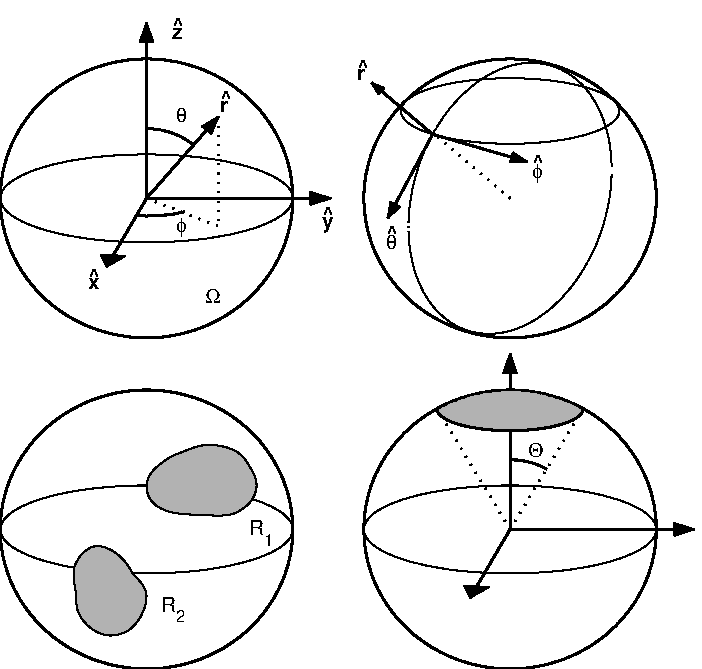
\includegraphics[width=0.5\textwidth]{figures/psdiagram.pdf}
  \caption{\label{coordsys} The Cartesian and spherical
    coordinate systems and the directions of the magnetic field
    components (upper panels), and regions on the planet's surface.}
\end{figure}


\subsection{Data variables and format}
The programs \verb+LocalIntField+ and \verb+LocalIntExtField+ require
the data described in table~\ref{datatable}.

\begin{table}
  \caption{\label{datatable} Data required by the programs
    \texttt{LocalIntField} and \texttt{LocalIntExtField} }
  \centering
  \begin{tabular}{l|l}
    Array&Description\\
    \hline
    \verb+lon+&Longitudinal position of the data point [radians]\\
    \verb+cola+&Colatitudinal position of the data point [radians]\\
    \verb+r+&Radial position of the data point \\
    &[km away from center of Mars]\\
    \verb+data+& Radial (\verb+data{1}+), colatitudinal (\verb+data{2}+),\\
    &and longitudinal (\verb+data{3}+) magnetic field component [nT]\\
  \end{tabular}
\end{table}


Besides the variables described in table~\ref{datatable}, you need to
choose values for the following variables:

\texttt{dom}: The region. This can be either a named region for which
you have an m-file that provides lon/lat coordinates (see for example
\texttt{namerica.m}) or it can be a spherical cap or spherical ring
(the area between two spherical caps). If you want a spherical cap,
set \texttt{dom} as the semi-opening angle $\Theta$ of the cap (see
figure~\ref{coordsys} bottom right panel). If you want a spherical
ring, provide the two semi-opening angle. If your sperical cap/ring
are not centered on the north pole, you will also have to provide the
longitude/latitude of the center (\texttt{rotcoord}). See the help
page of \texttt{LocalIntField} and \texttt{LocalIntExtField} for more
detail.

\texttt{LmaxIn}: Maximum spherical-harmonic degree \verb+LmaxIn+
for the internal field, or two degrees\\ \verb+[LmaxIn(1) LmaxIn(2)]+, if
you want the internal field to be calculated for the spherical
harmonics between (and including) \verb+LmaxIn(1)+ and \verb+LmaxIn(2)+.

\texttt{LmaxOut}: Maximum spherical-harmonic degree for the external
field.

\texttt{J}: Number of Slepian functions you want to use to calculate
the solution. Too few means that the solution does not resolve as much
as the data would allow. Too many means that you start creating
artifacts in the solution. There are strategies to find an optimal
solution. We will describe these later.

\texttt{rplanet}: Radius of the planet (we assume that the planet is a
perfect sphere. You can use the average radius in the region that you
are investigating.) 

For \verb+LocalIntExtField+ you also need to provide the two variables


\texttt{LmaxOut}: Maximum spherical-harmonic degree for the external
field.

\texttt{router}: Maximum radial position of the satellite; radial
position for external field.

There are more variables that can/should be chosen. Check out the help
pages of \texttt{LocalIntField} and \texttt{LocalIntExtField}.


\section{Obtaining raw data}

NASA provides planetary magnetic data for all past and current missions on their Planetary Data System (PDS) website \url{http://pds.nasa.gov/}. Often, these data sets come in the cartesian coordinate system and may need to be transformed into the spherical coordinate system, including the magnetic field components. For this purpose you can use the function \texttt{MAGcart2sph.m}. The folder \verb+slepian_hotel/MGS/+ contains additional programs to load and organize PDS data files for Mars Global Surveyor magnetic data. But they can be adapted for other data sets.


%% Mars Global Surveyor data (for example the pre-mapping data) can be downloaded from {\url{http://pds.nasa.gov/}} if you follow the links through ``Mars'', ``Mars Global Surveyor'', ``Magnetometer'', ``MGS MARS MAG/ER PRE-MAP MAG FULL WORD RESOLUTION V1.0'', ``Planetary Plasma Interactions Website'' and then click on the download button. You can obtain the Mapping data ``MGS MARS MAG/ER MAPING MAG FULL WORD RESOLUTION V1.0'' in the same way. The data folders are relatively large (pre-mapping: 8.5 GB, mapping: 20 GB).
 
%% Once you downloaded the data you can move all data files into one single folder using \\  \verb+PreparingMappingPhase.m+ 
%% and then read into Matlab/Octave using \verb+loadmanypds.m+. Once the files are in Matlab/Octave format, you can transform them into longitude, colatitude, radial format and extract locations over selected spherical cap regions using \verb+MAGcart2sph.m+

%% \section{Data structure and programs}
%% Programs for extracting, analyzing, and plotting the data are in the folder ``MGScodes''. In this section and the following sections I will explain, based on an example subset how to use these and other codes to analyze and plot the MGS data.

%% The entire MAG data set collected by Mars Global Surveyor is around 30GB large. Much too much to work with easily. Also, we often are only interested in a small subset. For example, if we only investigate a specific region on the globe, we don't need the data on the rest of the planet. Also, in some investigations we might want to look at only nighttime data, or only daytime data, or only low altitude data, or only high altitude data, etc.

%% I already extracted data locations over 4 specific named regions such as the entire South Polar region (south of latitude -76), Prometheus Planum, Australe Montes, and Southern Terra Sirenum.

%% These regions seem appropriate because they offer a wide range of crustal magnetic field strengths. See my paper for reference.

%% If you load for example the data set \verb+premapping_SouthPole76.mat+, you have the entire data set that Mars Global Surveyor collected south of Latitude $-76$ during it's pre-mapping phase. The premapping phase contains data at strongly varying altitudes. 

%% The transformed data in \verb+premapping_SouthPole76.mat+ and other prepared data sets contain a number of variables. Most of these variables are arrays (vectors) of equal length, where the $n$-th entry corresponds to the $n$-th data point. The following array summarizes the most important arrays

%% \begin{tabular}{l|l}
%% Array&Description\\
%% \hline
%% \verb+lon+&Longitudinal position of the data point [radians]\\
%% \verb+cola+&Colatitudinal position of the data point [radians]\\
%% \verb+r+&Radial position of the data point \\
%% &[km away from center of Mars]\\
%% \verb+data+& Radial (\verb+data{1}+), colatitudinal (\verb+data{2}+),\\
%% &and longitudinal (\verb+data{3}+) magnetic field component [nT]\\
%% \verb+sao+& Solar energy collected by the solar panels [Am]\\
%% \verb+date+& Year, day of year, hour, minute, second, \\
%% &and millisecond when the data was collected
%% \end{tabular}

%% For example, \verb+cola(10)+ contains the the colatitude (in radians) of the 10th data point in the data set you loaded. If you want to display the value of the latitude in degrees, try

%% \qquad \verb+90 - 180/pi*cola(10)+

%% This gave us the latitude of that specific data point. The same data point has longitude \verb+180/pi*lon(10)+. The factor \verb+180/pi+ is necessary to go from radians to degrees. If you want to plot the entire distribution of data points try

%% \qquad \verb+plot(180/pi*lon,90 - 180/pi*cola(10),'x')+

\section{Extracting data subsets}


\HERE

Let's see how the altitude of the data points is distributed. if you run

\qquad \verb+plot(r)+

you will see the radial position of the satellite plotted against the data point number. The altitude values (y-axis) show the distance from the Martian center. To get an idea of how high above the surface the satellite was, you can run \verb+plot(r-3390)+. The number 3390 is the mean volumetric radius of Mars. Of course, in order to get the exact altitude, you would need to subtract both the geoid height and the topography on top of geoid. (Geoid is explained here: \url{https://www.youtube.com/watch?v=q65O3qA0-n4}).


When looking at the previous plotting result you will see that there was a short time when the altitude was very low.  If you want to find the indices (data entry numbers) of data locations that are very low altitude, use Matlab/Octave's \verb+find+ command. For example, if you want to find data that is below 200 km above the Mars mean volumetric radius of 3390 km you can run

\qquad \verb~indices=find(r<3390+200);~

Of course you could have replaced 3390+200 by 3590. You can check the number of entries in indices by running \verb+length(indices)+. It will show that indices has 12568 data entries. This compares to \verb+length(r)+ which shows 1855344 entries. This means that only 12568 out of the 1855344 data points measured over the South Polar region during the prompting phase were measured below 200 km altitude above mean average radius 3390.

If we now want to throw out all the data points that were collected above those 200 km we can do that by saying for example 

\qquad \verb+r=r(indices)+

Now you only kept the data point numbers indicated by the variable ``indices'' and deleted everything else. To throw out all higher altitude data points at all other arrays as well you need to run 

\qquad \verb+lon=lon(indices);+

\qquad \verb+cola=cola(indices);+

\qquad \verb+data{1}=data{1}(indices);+

\qquad \verb+data{2}=data{2}(indices);+

\qquad \verb+data{3}=data{3}(indices);+

\qquad \verb+date=date(indices,:);+

and so on for every array. It is best to write an m file that does this so you can be sure you did it for every variable and it is easy to reproduce it. I wrote the script \verb+cutDataScript.m+ that does just that.


The array \verb+sao+ contains the solar panel output of the satellite. you can check out the solar panel readings by running

\qquad \verb+plot(sao)+

Some of the data points have large values, others have value zero or negative. The value -99 means that the solar array output was zero or negative, which means the panels were not illuminated by the sun. The value -999 would mean that no solar panel data is available for that data point. Run \verb+find(sao==-999)+ (the double = sign is necessary to tell Ocatve/Matlab that you want to compare two numbers and not assign a value to a variable) to see that there is no data point without a solar panel reading.

We now filter out the data points where the solar panels where lit. Run

\qquad \verb+indices=find(sao<=0);+

This will give you a new set of indices. From all the data points that were at low altitude, we now only retain the ones, where the satellite was in darkness. Run your script that contains \verb+r=r(indices)+ etc to retain only nighttime, low altitude data.

Save the data subset that you just created, give it an appropriate name that reflects what exactly you did to obtain it.

Use similar approaches to obtain for example high altitude nighttime data, low altitude daytime data, etc. Get the subset from different satellite phases: premapping, mapping in 1999, mapping in 2000, etc. You can also combine different data sets by simply appending them. For example if \verb+r_map1999+ is the radial position for the mapping phase in 1999 and \verb+r_map2000+ is the radial position for the mapping phase in 2000, you can get the radial position array that forst has all the 1999 and then all the 2000 radial positions by running

\qquad \verb+r=[r_map1999;r_map2000];+

Do this with all arrays (e.g. \verb+data{1}=[data_map1999{1};data_map2000{1}];+ etc.) and you have your new combined data set.

Again, save that data set with an appropriate name and precise notes on how you obtained it. Or you can write an m file that reproduces exactly your data selection.

\section{Plotting models described by coefficients}\label{plotting single alt}


If you have a coefficients from a magnetic model and you want to plot them, follow the instructions in this section. You can invert for your own model coefficients following the instructions in section~\ref{repro}. 

The coefficients are usually either coefficients for scalar- or vector spherical-harmonics. You can plot the corresponding model by expanding the coefficients as a linear combination of the scalar- or vector spherical harmonics. Here we call the scalar spherical harmonics $\Yfun_{lm}$ and the vector spherical harmonics $\Efun_{lm}$. See my paper for more detail. 

You can calculate linear combinations of scalar spherical harmonics using \verb+plm2xyz+ and linear combinations of vector spherical harmonics using \verb+elm2xyz+. I will explain how that works in a moment but first we will need to talk about coefficient ordering schemes.


Programs such as \verb+LocalInnerField+, or the matrices that come out of \verb+glmalpha+ return spherical-harmonic coefficients in vector form. In our codes  we use two different ways of ordering the spherical harmonic coefficeints: ADDMOUT and ADDMON. 

Remember that spherical harmonics have a degree $l$ and an order $m$. degrees are all integers greater than zero and orders for each degree vary between $-l$ and $l$.

We could order these spherical harmonics as


\begin{tabular}{c|cccccccccc}
l&0&1&1&1&2&2&2&2&2&etc.\\
\hline
m&0&-1&0&1&-2&-1&0&1&2&\text{etc.}
\end{tabular}

This is called the ADDMOUT ordering and is the ordering in which the columns of the Slepian matrices in \verb+glmalpha+, \verb+gradvecglmalpha+, and all these other similar functions are returned.

The other ordering that we are using is:

\begin{tabular}{c|cccccccccc}
l&0&1&1&1&2&2&2&2&2&\text{etc.}\\
\hline
m&0&0&-1&1&0&-1&1&-2&2&\text{etc.}
\end{tabular}

This one we call ADDMON and it is the ordering in which the coefficients from functions like \verb+LocalInnerField+ are returned. Every function that returns coefficients or matrices of coefficients should state in their help menu in which format the coefficients are.

Luckily there is a neutral type of sorting that is often used once the coefficients are calculated: LMCOSI

In the lmcosi format, we explicitly write out the degrees, orders, and coefficients which in the following I will call $c_{l\,m}$

\begin{tabular}{c c c c}
l&m&co&si\\
\hline
0&0&$c_{0\,0}$&0\\
1&0&$c_{1\,0}$&0\\
1&1&$c_{1\,-1}$&$c_{1\,1}$\\
2&0&$c_{2\,0}$&0\\
2&1&$c_{2\,-1}$&$c_{2\,1}$\\
2&2&$c_{2\,-2}$&$c_{2\,2}$\\
\vdots&\vdots&\vdots&\vdots
\end{tabular}

As you can see this last ordering is an entire matrix instead of just a vector. This is a disadvantage to run calculations but it is less ambiguous than just a vector of coefficients.


Luckily we have programs that take care of these issues. These programs have the creative names
\verb+coef2lmcosi+ and \verb+lmcosi2coef+. You can probably guess from the name what each does.

Now load the coefficients for one of the crustal magnetic field models that either you obtained from me, or that you calculated yourself. For example, take\\ \verb+L130_200night_r3376_avgalt135_J620_weighres.mat+.\\ 
You can load it by typing

\qquad \verb+load 'L130_200night_r3376_avgalt135_J620_weighres.mat'+

This will load a vector named \verb+coef+ of length 17161, which is $(130+1)^2$ and a few other variables. The vector is in addmon format, because it came from \verb+LocalInnerField+. 

The coefficients that you just loaded are coefficients for the magnetic potential. You can turn them into coefficients of the magnetic field by calculating the derivative of the magnetic potential field. The function \verb+vecupderivative+ does that for you. You can also give it a different radius if you want to calculate the magnetic field for example at an average satellite altitude. For the Martian South Pole let's choose the altitude to which we want to continue the field as \verb+viewalt=3376+. The radius to which the coefficients were normalized is \verb+MarsPolRad=3376+ (see the filename of the file that I stored the coefficients in). Run

\verb+coefB=vecupderivative(coef,viewalt,MarsPolRad,130);+

We now turn it into the lmcosi format by running

\qquad \verb+lmcs=coef2lmcosi(coefB);+

I just name the output \emph{lmcs} but you can give it any name you want. If coef had been in addmout format you would have needed to give \verb+coef2lmcosi+ an additional 1 such as \verb+coef2lmcosi(G(:,ind),1)+. See the help part of \verb+coef2lmcosi+ for more detail.

You can evaluate the coefficients for the vector spherical harmonics $\Efun_{lm}$ that are stored in \emph{lmcs} on the planet's surface by running 

\qquad\verb+[datasim,lon,lat]=elm2xyz(lmcs,res);+

You need to choose a value for \emph{res}. It gives the resolution plot. You can choose \emph{res}=1, or 0.5, or even 0.1 to get a very high res image. But it will also use much calculation time and memory.

To plot the radial component of the solution run 

\qquad\verb+plotplm(datasim{1},lon*pi/180,lat*pi/180,2);+

This will give you a 3D sphere that you will need to rotate because the model is mostly on the South pole. You can replace the number 2 in the above command to get different map stiles.

Rotate the sphere either with your mouse or click on ``R'' or the rotate symbol in the figure or run

\qquad\verb+view(90,-90)+

to view the South Pole.

The output doesn't show much and has strong wiggles away from the South Pole. This is because the solution needed to fit strong field variations within the Southpole but is unconstrained outside of the South Polar area. Run

\qquad\verb+colorbar+

To see the plotted range and adjust it to

\qquad\verb+caxis([-20000 20000])+

Now the area outside the South Pole goes haywire but within the South Pole you see a bit something. Set the color scheme to something more appropriate, run 

\qquad\verb+ampcol+

and 

\qquad\verb+colorbar+
%\qquad\verb+kelicol(1)+

Still not a very nice plot but it does the trick.

If you actually want to make beautiful plots, use GMT \\(http://gmt.soest.hawaii.edu/). See section~\ref{OctaveGMT} for instructions on how to export data to GMT.

\textbf{Exercise:} Plot this field at satellite altitude 100 km above radius 3376 km. Select your own value range for the color bar to make it look ok. 

\textbf{Exercise:} Plot this field at satellite altitude 200 km above radius 3376 km. Select your own value range for the color bar to make it look ok. 

\textbf{Question:} What do you observe? How does the field change when you go to higher altitudes?

\section{Evaluating a model at varying satellite altitude}


Let's say you want to compare the model described by a set of spherical-harmonic coefficients to a set of data points that were collected by the satellite. These ``real'' data points are each at an individual altitude. In section \ref{plotting single alt} you learned how to plot the models at a single altitude, but this won't help much if you want to know exactly how different the modeled value at each individual point is from the measured value. 

Luckily we have a function that does that: \verb+rGvec+ 
 What you need in order to use this function is: the coefficients (in addmon format) \emph{coef}, the data point locations (longitude \emph{lon}, colatitude \emph{cola}, radial position \emph{r}), and the reference radius of the planet for the spherical-harmonic coefficients \emph{planet}. For example if you load the coefficients from model\\
  \verb+L130_200night_r3376_avgalt135_SouthernTerraSirenum_J90_weighres.mat+,\\
and the corresponding data from \verb+premapping_SouthernTerraSirenum.mat+, you can evaluate the modeled data values for the coefficients at exactly the same locations and altitudes as the measured satellite data by running

\qquad \verb+moddata=rGvec(coef,cola*pi/180,lon*pi/180,r,3376);+

The reference radius 3376 km is what was used as the planet's radius when I originally calculated the model (as is indicated in the filename). The calculation will take a while. Save the modeled data after calculation!

As a first check to see if the modeled data and the evaluated data are even close to being similar you can just plot for example the radial component of the magnetic field of both data sets:

\qquad \verb+plot(data{1})+

to plot the radial component satellite data, then

\qquad \verb+hold on+

\qquad \verb+plot(moddata{1},'r')+

to plot the modeled data on top of it. It looks quite similar but not exactly. This is what we would expect. We are fitting the 739 data locations (and therefore 2217 data values) with only 90 different Slepian functions. 

If you want to make the same comparison for the latitudinal and the longitudinal components, do the same with \verb+data{2}+, \verb+moddata{2}+ and  \verb+data{3}+, \verb+moddata{3}+.

Of course this does not plot the data in their spatial locations but just ordered in the sequence the satellite measured them. We might want to know where exactly the errors are large. To do that, we have the function \verb+plotSouthpole.m+. Say you want to plot the radial component of the data, run 

\qquad \verb+plotSouthpole(data{1},lon,cola)+

Of course you will need to adjust the color scale. First, choose for example

\qquad \verb+kelicol(1)+ 

and then set the color scheme to be symmetric for example between -400 and 400 nT:

\qquad \verb+caxis([-400 400])+


\textbf{Exercise:} Plot the difference between the modeled and the measured data. Is there a systematic error? Or is the error in individual measurements that are seemingly random?

\textbf{Exercise:} For the same region, prepare another data set, for example higher altitude nighttime. Use the same approach as described earlier to extract the data set from for example some year of the mapping phase. Save the extracted data before proceeding for reproducibility and save every step you do in an m-file.




 







\section{Reproducing my models from the data sets}\label{repro}
The description in this section will give you a model that is close to but not exactly my model for the entire South Polar region. To get exactly the same model you need to get all the data from the premapping phase that is South of latitude $-74.5^\circ$ and then continue as described below.

Load the pre-mapping South Polar data. Retain the low altitude data points and then retain the nighttime data points just as described earlier. You can reproduce model SP130 by running

\qquad \verb+coef=LocalInnerField(data,...+\\
\verb+r,cola,lon,[166 177],130,620,3390,3525,[0 -90]);+

You can look up what the individual numbers that I gave the program mean by running

\qquad \verb+help LocalInnerField+

The ... tells Octave/Matlab that the command continues on the next line

If you decide to reproduce my results, the first time running this will be quite slow because the program first needs to calculate the Slepian functions. Once they are calculated, it will be much much faster.

When you compare these results to my model SP130 you will see that they look slightly different but not by much. This is because I included a few points outside of the region into my calculations.


\section{Writing GMT files with Octave}\label{OctaveGMT}

If you are using Octave, you will need to install NetCDF or load the package if it is installed. If you have Matlab you already have that installed and ready. If you are using Octave on a Mac and you installed it like described in the intro document, then you will need to add netcdf. 
Luckily this is very easy with Octave's package installer: just run

\qquad\verb+ pkg install -forge netcdf+

and you have it. I wrote the loading of the package into the calling functions so you don't even need to worry about loading the package.

You can export your field to a GMT format using \verb+GMTexportfield+ see the help part of the function for how to use it. Of course you will need to download, install, and learn GMT to then plot it. I will provide useful scripts but we leave that for another time.


\end{document}
